%\documentclass[letterpaper,12pt]{article}

\documentclass[10pt]{book}

%-- imports
% QRK
\newcommand{\runDate}{202007}
\newcommand{\multipleNum}{7}
\newcommand{\projectNum}{9}
\newcommand{\iterationNumber}{1}

% Set Specific Variables
\newcommand{\setNumberStart}{0}
\newcommand{\setNumberEnd}{20}
\newcommand{\cardNumberStart}{1}
\newcommand{\cardNumberEnd}{20}

% Card Size
\newcommand{\cardHeight}{4}
\newcommand{\cardWidth}{5.5}


% page dimensions
\newcommand{\halfHeight}{2.125} %1.9 for box!
\newcommand{\halfWidth}{2.75}  %2.8

% --- Packages
\usepackage[paperwidth= \cardWidth in, paperheight=\cardHeight in,top=0in, bottom=0in, left=0in, right=0in]{geometry}

\usepackage{tikz} 			%draw

\usepackage{fontspec}		%Set font
\setmainfont{Orbit}           % special by Evan Pittson Design

\usepackage{ifthen}			% if then else

\usepackage{mathtools}

% --- Formatting
\pagenumbering{gobble}
\setlength{\parindent}{0pt}


% --- Variables
\newcommand{\topLineY}{2.75}
\newcommand{\lineLeft}{6.25}
\newcommand{\nextIncrement}{\lineLeft+0.25}
\newcommand{\lineLength}{3.5}
\newcommand{\lineEnd}{\lineLeft+\lineLength}
\newcommand{\lineSpacing}{0.65}

\newcommand{\topAddressL}{6.5}
\newcommand{\topAddressT}{3}
\newcommand{\bottomAddressL}{0.1}
\newcommand{\bottomAddressT}{3}
\newcommand{\addressGap}{0.5}
\newcommand{\addressLength}{3.4}

\newcommand{\stampGreyPercentage}{10}

\begin{document}
	\foreach \card in {1,2,...,20}
	{
		\ifthenelse{\card=19}
		{
			% card 19's back
			\begin{center}
				\begin{figure}
					\resizebox{\paperwidth}{\paperheight}
					{\begin{tikzpicture}[]	

% dividing line
\draw[line width = 0.005cm,fill=black!30!white]
		(8,3.5) to (2,1.5);

% corner points
\node [] at (0,0) {\includegraphics[scale=0.05]{logo.png}};
\node [] at (0,5) {\includegraphics[scale=0.05]{logo.png}};
\node [] at (10,0) {\includegraphics[scale=0.05]{logo.png}};
\node [] at (10,5) {\includegraphics[scale=0.05]{logo.png}};

% lines
\draw[line width = 0.005cm,fill=black!30!white]     (\lineLeft,\topLineY) to (\lineLeft+\lineLength,\topLineY);
\draw[line width = 0.005cm,fill=black!30!white] (\lineLeft,\topLineY-\lineSpacing) to (\lineLeft+\lineLength,\topLineY-\lineSpacing);
\draw[line width = 0.005cm,fill=black!30!white] 	(\lineLeft,\topLineY-2*\lineSpacing) to (\lineLeft+\lineLength,\topLineY-2*\lineSpacing);

% stamp corner UR
\foreach \num in {8.666,9.333}
    \node [anchor=center] at (\num, 5) {\includegraphics[scale=0.05]{logo.png}};
\foreach \num in {8,8.666,9.333}
	\node [anchor=center] at (\num, 3.5) {\includegraphics[scale=0.05]{logo.png}};
	
\foreach \num in {3.8,4.1,4.4,4.7,5}
	\node [anchor=center] at (8,\num) {\includegraphics[scale=0.05]{logo.png}};
\foreach \num in {3.5,3.8,4.1,4.4,4.7}
	\node [anchor=center] at (10,\num) {\includegraphics[scale=0.05]{logo.png}};
	
% center UR
\node [anchor=center] at (9, 4.25) {\includegraphics[scale=0.05]{logo.png}};

% stamp corner BL
\foreach \num in {8.666,9.333}
    \node [anchor=center] at (\num, 5) {\includegraphics[scale=0.05]{logo.png}};
\foreach \num in {8,8.666,9.333}
	\node [anchor=center] at (\num, 3.5) {\includegraphics[scale=0.05]{logo.png}};
	
\foreach \num in {0.3,0.6,0.9,1.2,1.5}
	\node [anchor=center] at (0,\num) {\includegraphics[scale=0.05]{logo.png}};
\foreach \num in {0,0.3,0.6,0.9,1.2}
	\node [anchor=center] at (2,\num) {\includegraphics[scale=0.05]{logo.png}};

% center BL
\node [anchor=center] at (1, 0.75) {\includegraphics[scale=0.05]{logo.png}};

\end{tikzpicture}}
				\end{figure}
			\end{center}
		}
		{  % normal card backs
			\begin{center}
				\begin{figure}
					\resizebox{\paperwidth}{\paperheight}
					{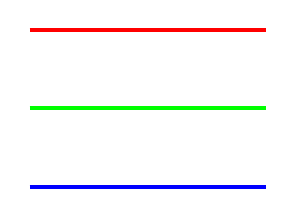
\begin{tikzpicture}[]	



\draw[red,line width = 0.05cm] (2,3) to (5,3);
\draw[green,line width = 0.05cm] (2,2) to (5,2);
\draw[blue,line width = 0.05cm] (2,1) to (5,1);

\end{tikzpicture}}
				\end{figure}
			\end{center}
		}
	}
\end{document}